\documentclass[margin,line,11pt]{resume}
 
\usepackage[latin1]{inputenc}
\usepackage[english,french]{babel}
\usepackage[T1]{fontenc}
\usepackage{fontawesome}
\usepackage{graphicx,wrapfig}
\usepackage{url}
\usepackage[colorlinks=true, pdfstartview=FitV, linkcolor=blue, citecolor=blue, urlcolor=blue]{hyperref}
\pdfcompresslevel=9


\begin{document}{\sc \Large Qiang Meng}
\begin{resume}

% === PICTURE ===

    \vspace{0.5cm}
    \begin{wrapfigure}{R}{0.15\textwidth}
         \vspace{-0.9cm}
        \begin{center}
        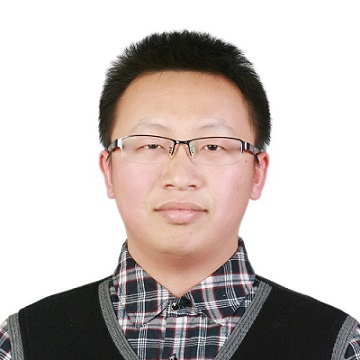
\includegraphics[width=0.11\textwidth]{face}
        \end{center}
         \vspace{-1cm}
    \end{wrapfigure}

% === PERSONAL INFO ===
 
    \section{\mysidestyle Contact\\Information}
    \textbf{Email}:\hspace{1.5em}\quad  IrvingMeng@outlook.com \\
    \textbf{Phone}: \hspace{1.5em} (206)-409-4201\\ 
    \textbf{Address}: \hspace{1em}9522 1st Ave NE Apt B6\\
     \hspace*{6em}Seattle, WA, 98115 

    \section{\mysidestyle  Objective}
 To obtain a full-time position in the field of machine learning and data science, applying my knowledge in machine learning, artificial intelligence, optimization, and programming.
      

     \section{\mysidestyle Education}
     \textbf{University of Washington  \hfill WA, USA}\\
Ph.D. Candidate \quad  Industrial and System Engineering \hfill \textit{Sep 2015 - present}\\
 GPA: 3.7/4.0 \par

 \textbf{University of Science and Technology of China \hfill Hefei, China}\\
 B.S. \quad Mechanical Engineering \hfill \textit{Jun 2015}\\
 GPA: 3.78/4.3 (Rank: 3/61)
           
% === OBJECTIVE ===

    % \section{\mysidestyle Professional Objective}
    % Improve the efficiency of the microwave and RF designers and structures. I focus on nonlinear devices at circuits level (such as HEMTs transistors) and at system level (HPA, Switches). That purpose requires an original use of an advanced RF instrumentation associated to a strong knowledge in terms of measured devices modeling.
 
% === SKILLS ===
     

% === AWARDS ===

        \section{\mysidestyle Honors}
        \begin{list2}
        \item {Teaching Assistant, University of Washington, 2016-2018}
                \item {College of Engineering Dean's Fellowship, University of Washington, 2015-2016}          
        \item {Samsung Scholarship , University of Science and Technology of China, 2014-2015}
        \item {National Encouragement Scholarship, University of Science and Technology of China, 2013-2014}
        \item {First prize in the Challenge Cup, USTC, 2013}          
        \item {National Encouragement Scholarship, University of Science and Technology of China, 2012-2013}          
        \item {1st place in RoboGame Robot Competition, USTC, 2012}
        \end{list2}

        \section{\mysidestyle Publications}
        Huang, Y., \textbf{Meng, Q.}, Evans, H., Lober, W., Cheng, Y., Qian, X., Liu, J. and Huang, S., 2017. CHI: A contemporaneous health index for degenerative disease monitoring using longitudinal measurements. Journal of biomedical informatics, 73, pp.115-124.\par
       \textbf{Meng, Q.} and Simge, K. , Use mixed-integer optimization to select features under trace ratio criterion combining redundancy constraints and prior knowledge. [\textbf{In progress}]
        
        \section{\mysidestyle Selected Courses (Graduate-Level)}
\vspace{0.5em}
	\begin{tabular}{ll }
          \textbf{Machine Learning} & Machine Learning; Big Data; Artificial Intelligence; Graphical Model; \\
                           &  Non-parametric Process; Markov Decision Process\\
  \textbf{Optimization} & Linear, Integer Programming; Convex,  Global Optimization \\
   \textbf{Statistics}& Statistical Inference; Statistical Computing; Time Series \\
\textbf{Quality Engineering} & Quality Control; Design of Experiments \\
	\end{tabular}

 

% \section{\mysidestyle Selected Projects}
%         \begin{list2}
% \item	3 years' professional experience with analytics in digital advertising and sales/marketing fields.
% \item	Proficient in data ETL, visualization, analyzing and modeling with SQL, Excel/VBA, Tableau, Python and R.
% \item	Experienced in designing and conducting strategic projects to identify opportunities for improvements.
% \end{list2}

        \section{\mysidestyle Teaching Experience}
        \begin{list2}
        \item   Probability and Statistics for Engineers; Spring, Summer 2017, Winter, Spring 2018 
        \item   Linear and Network Programming; Autumn 2016, Autumn 2017
        \item  Fundamentals of Engineering Economy; Winter 2016
        \end{list2}
        
 \section{\mysidestyle Skills}
\vspace{0.5em}
	\begin{tabular}{ll }
\textbf{Programming languages} &Python, Matlab, C++, R, Julia, Caffe\\
\textbf{Scientific softwares}& Labview,  AutoCAD, OpenCV\\
	\textbf{Tools}& Linux, Emacs, Git, \LaTeX, Hadoop
        \end{tabular}

\clearpage        

\section{\mysidestyle Selected Project}

        \textbf{Feature Selection Combining Redundant Information and Prior Knowledge}
\begin{list2}        
\item Proposed a Mixed-integer model which can select novel features which contain less redundancy and fit well with prior knowledge.
\item Digged into the structure of the optimal solutions. Provided several ways to speed up the solving process.  These speed-up methods worked well especially with big data.
\item Theoretically analyzed the NP-hard problem and proved  that this problem is polynomial-solvable under certain conditions. 
\item The existing experimental results showed better performances over traditional feature selection methods in the machine learning area. \textbf{[In progress]}
\end{list2}

\textbf{Contemporaneous Health Index}
\begin{list2}        
\item Developed a novel formulation for contemporaneous patient risk monitoring. This formula translated multivariate longitudinal measurements into a contemporaneous health index (CHI) that captures patient condition changes over the course of progression. The formulation can work in both supervised and unsupervised manner. 
\item Proposed  algorithms to mitigate the challenges associated with the nonsmooth convex optimization problem. Our algorithms involved dual reformulation and block coordinate descent. Extensive numerical studies were performed on both synthetic datasets and real-world applications on Alzheimer's disease and Surgical Site Infection.
\end{list2}

\textbf{Interesting Course Projects Related to Machine Learning}
\begin{list2}
\item \textbf{Sparse Principle Component Analysis (sPCA)}. Proposed an algorithm combining alternating maximization (AM) method and convex optimization to solve the NP-hard problem. Only a few explained variances were sacrificed and the orthogonality of PCs were guaranteed. 
\item \textbf{Training neural networks with Particle Swarm optimization (PSO)}. A global optimization method called PSO was used to search for the optimal parameters of a neural network.  Its performances were compared with the traditional gradient methods.
% \item \textbf{Parameter tuning of deep neural network}. Played with the CNN on CIFAR data-set with Caffe. 
\item \textbf{K kernel nearest-neighbor algorithm for the Netflix competition}. Implemented kNN, Kernal kNN, weighted kNN for the Netflix competition. $k$ was found by leave-one-out cross validation. 
\item \textbf{Scaling up K-Means with MapReduce}. Implemented the k-means algorithm in Hadoop MapReduce to cluster the BBC News with the TF-IDF values.
\item \textbf{PageRank with MapReduce}. Implemented the multiplication of big matrix with MapReduce to find the stationary distribution of the transition  matrix. 
\end{list2}


\textbf{Interesting Course Projects Related to Reinforcement Learning}
\begin{list2}        
\item \textbf{Cart-pole problem}. Implemented policy-based reinforcement learning  to solve for optimal movements which balance a pole connected with one joint on top of a moving cart. The performances of two learning methods (Monte-Carlo policy gradient and Actor-Critic policy gradient) are compared. 
\item \textbf{Kalah game}. Used minimax search with alpha-beta pruning as the basic algorithm. Proposed various heuristic functions and created different AIs to beat the basic AI. 
\end{list2}



\textbf{A Vision-based Intelligent Off-road Robot}
\begin{list2}
\item The leader and programmer of the team. Developed a real-time object recognition system (based on OpenCV) which navigated the robot by detecting  markers from the messy backgrounds. The system worked perfectly in the changeable out-door environment under various backgrounds and  weather conditions.
\item Designed the mechanical control system which could accurately complete the action of fetching a certain item and the action of climbing stairs.
\end{list2}






    	

 	

 	       
\end{resume}   
\end{document}